\documentclass[dvipdfmx]{jsarticle}
\usepackage{amsmath,amssymb}
%¥usepackage{mathpazo}
\usepackage{amsthm}
\newtheorem{dfn}{定義}
\newtheorem{thm}[dfn]{定理}
\newtheorem{lem}[dfn]{補題}
%\usepackage{newtxtext,newtxmath}
%\usepackage[hiresbb]{graphicx}
%¥図
\usepackage{bm}
%¥ボールド体
%\usepackage{mathrsfs}%ラグラジアン
\usepackage{wrapfig}%¥図の周りに文章を回り込ませる
\usepackage[dvipdfmx]{graphicx,color}
\usepackage{pgfplots}
\pgfplotsset{compat=1.16}
\usetikzlibrary{intersections,calc,arrows.meta,decorations.pathmorphing,backgrounds,positioning,fit,petri}
\usepackage{array}
\usepackage{siunitx}
\usepackage[version=3]{mhchem}
\usepackage{float}
\newcommand{\setN}{\mathbb{N}}
\newcommand{\setZ}{\mathbb{Z}}
\newcommand{\setQ}{\mathbb{Q}}
\newcommand{\setR}{\mathbb{R}}
\newcommand{\setC}{\mathbb{C}}
\usepackage{physics}
\usepackage{tcolorbox}
\usepackage[dvipdfmx]{hyperref}
\usepackage{pxjahyper}
\usepackage{tikz}
%\usepackage{gnuplot-lua-tikz}
\usepackage{subfigure}
\hypersetup{colorlinks=true}
\makeatletter
\@addtoreset{equation}{section}
\def\theequation{\thesection.\arabic{equation}}
\makeatother
\title{原子核物理 期末レポート} 
\author{Eymmetry \thanks{\url{https://twitter.com/Eymmetry}}}
\date{\today}
\begin{document}
\maketitle
\tableofcontents
\section{原子核の基本的性質}
\subsection{}\label{1-1}
自由な中性子の場合には$\beta$ 崩壊してより質量の軽い陽子になったほうが安定である。たいして原子核内ではWeizs\"{a}cker-Betheの質量公式によると1粒子あたりの結合エネルギーが
\begin{equation}
\label{eq:wi}
B(A,Z)=a_vA-a_sA^{\frac{2}{3}}-a_c \frac{Z^2}{A^{\frac{1}{3}}}-a_\text{sym} \frac{(N-Z)^2}{A}+\frac{\delta(Z,N)}{A^{\frac{1}{2}}}
.\end{equation}
でかけていてこれが$A=\mathrm{const}$のもと最小な条件を求めると
\[
Z=\frac{4a_\text{sym} }{a_c A^{\frac{2}{3}}+4a_\text{sym} }\frac{A}{2}
.\] 
となる(ここでペアリング項は無視した)。特に軽い原子核ではクーロン項も無視できて
\[
N\simeq Z\simeq  \frac{A}{2}
.\] 
のように陽子と中性子の数が大体等しいような数で$\beta$崩壊が起こらなくなる。
この起源は主にWeizs\"{a}cker-Betheの質量公式の対称項により、核子がフェルミオンであるので陽子と中性子の数が異なるとどちらかが多くなってエネルギー的に損してしまうから大体同じような数になっている。

なお重い原子核ではクーロン項が無視できなくなりそのために中性子が過剰になって来る。\\
\subsection{}\label{1-2}
\ref{1-1}のときに無視したペアリング項をいれて考える。ペアリング項は
\[
\delta(Z,N)=\begin{cases}
	+\SI{11.2}{MeV}& (\text{Z,Nがともに偶数})\\
	+\SI{0}{MeV}& (\text{Z,Nどちらかが偶数どちらかが奇数})\\
	+\SI{-11.2}{MeV}& (\text{Z,Nがともに奇数})\\
\end{cases}
.\] 
となりAが偶数の原子核に対してはZが偶数のほうが安定となる。
したがって例に上がっている同重体である$\mathrm{^{106}_{46}Pd}$や$\mathrm{^{106}_{48}Cd}$ はここから$\beta$崩壊すると Zが奇数になってしまって不安定になってしまうから$\beta$ 崩壊しない方が安定になる。このようにペアリング項を考えれば$\beta$ 崩壊に対して安定な原子核が複数存在しうる。\\
\subsection{}
ウランの原子番号は92であり、
$\mathrm{^{238}_{92}U}$は陽子の数も中性子の数も両方共偶数でありペアリング項の効果により安定である。
一方で$\mathrm{^{235}_{92}}$ は中性子の数が奇数であるのでペアを組むことができずに前者と比べると不安定になっている。したがってより安定な$\mathrm{^{238}U}$ の方が存在比が大きい。また$\mathrm{^{235}U}$ に中性子をあてて中性子が入ってくると一個ペアになれずに残っていた中性子も
ペアを組むことができてエネルギーが下がる。こうしてあまったエネルギーはすべて原子核全体の変形エネルギーに回されるため原子核はより激しく変形運動できることになり、核分裂もしやすくなる。一方で$\mathrm{^{238}U}$ だとすでにペアを組んでしまっているので新たな中性子が入ってきても前述のようなエネルギー収支上の旨味がないので核分裂は生じにくい。ただし高速な中性子の場合にはエネルギーがより高く中性子であるので核分裂が起こる。\\
\subsection{}
原子核の核模型にもとづいて議論する。
講義で扱ったようにエネルギー準位は
主量子数、方位量子数をつかって
\[
E_{nl}=\hbar\omega(2n+l+\frac{3}{2})=\hbar\omega(N+\frac{3}{2})
.\] 
と書くことができ、さらにここからスピン軌道相互作用によりエネルギー準位が分裂する(超微細構造)
。このとき

\[
E_{nlj}=(2n+l+\frac{3}{2})\omega+\begin{cases}
	-\frac{V_0^{\text{ls}}}{2}l &\left( j=l+\frac{1}{2} \right) \\
	+\frac{V_0^{\text{ls}}}{2}l &\left( j=l-\frac{1}{2} \right)
\end{cases}
.\] 
となり分裂した準位は$2j+1$ 個の状態を持つ。
\begin{figure}[H]
	\centering
	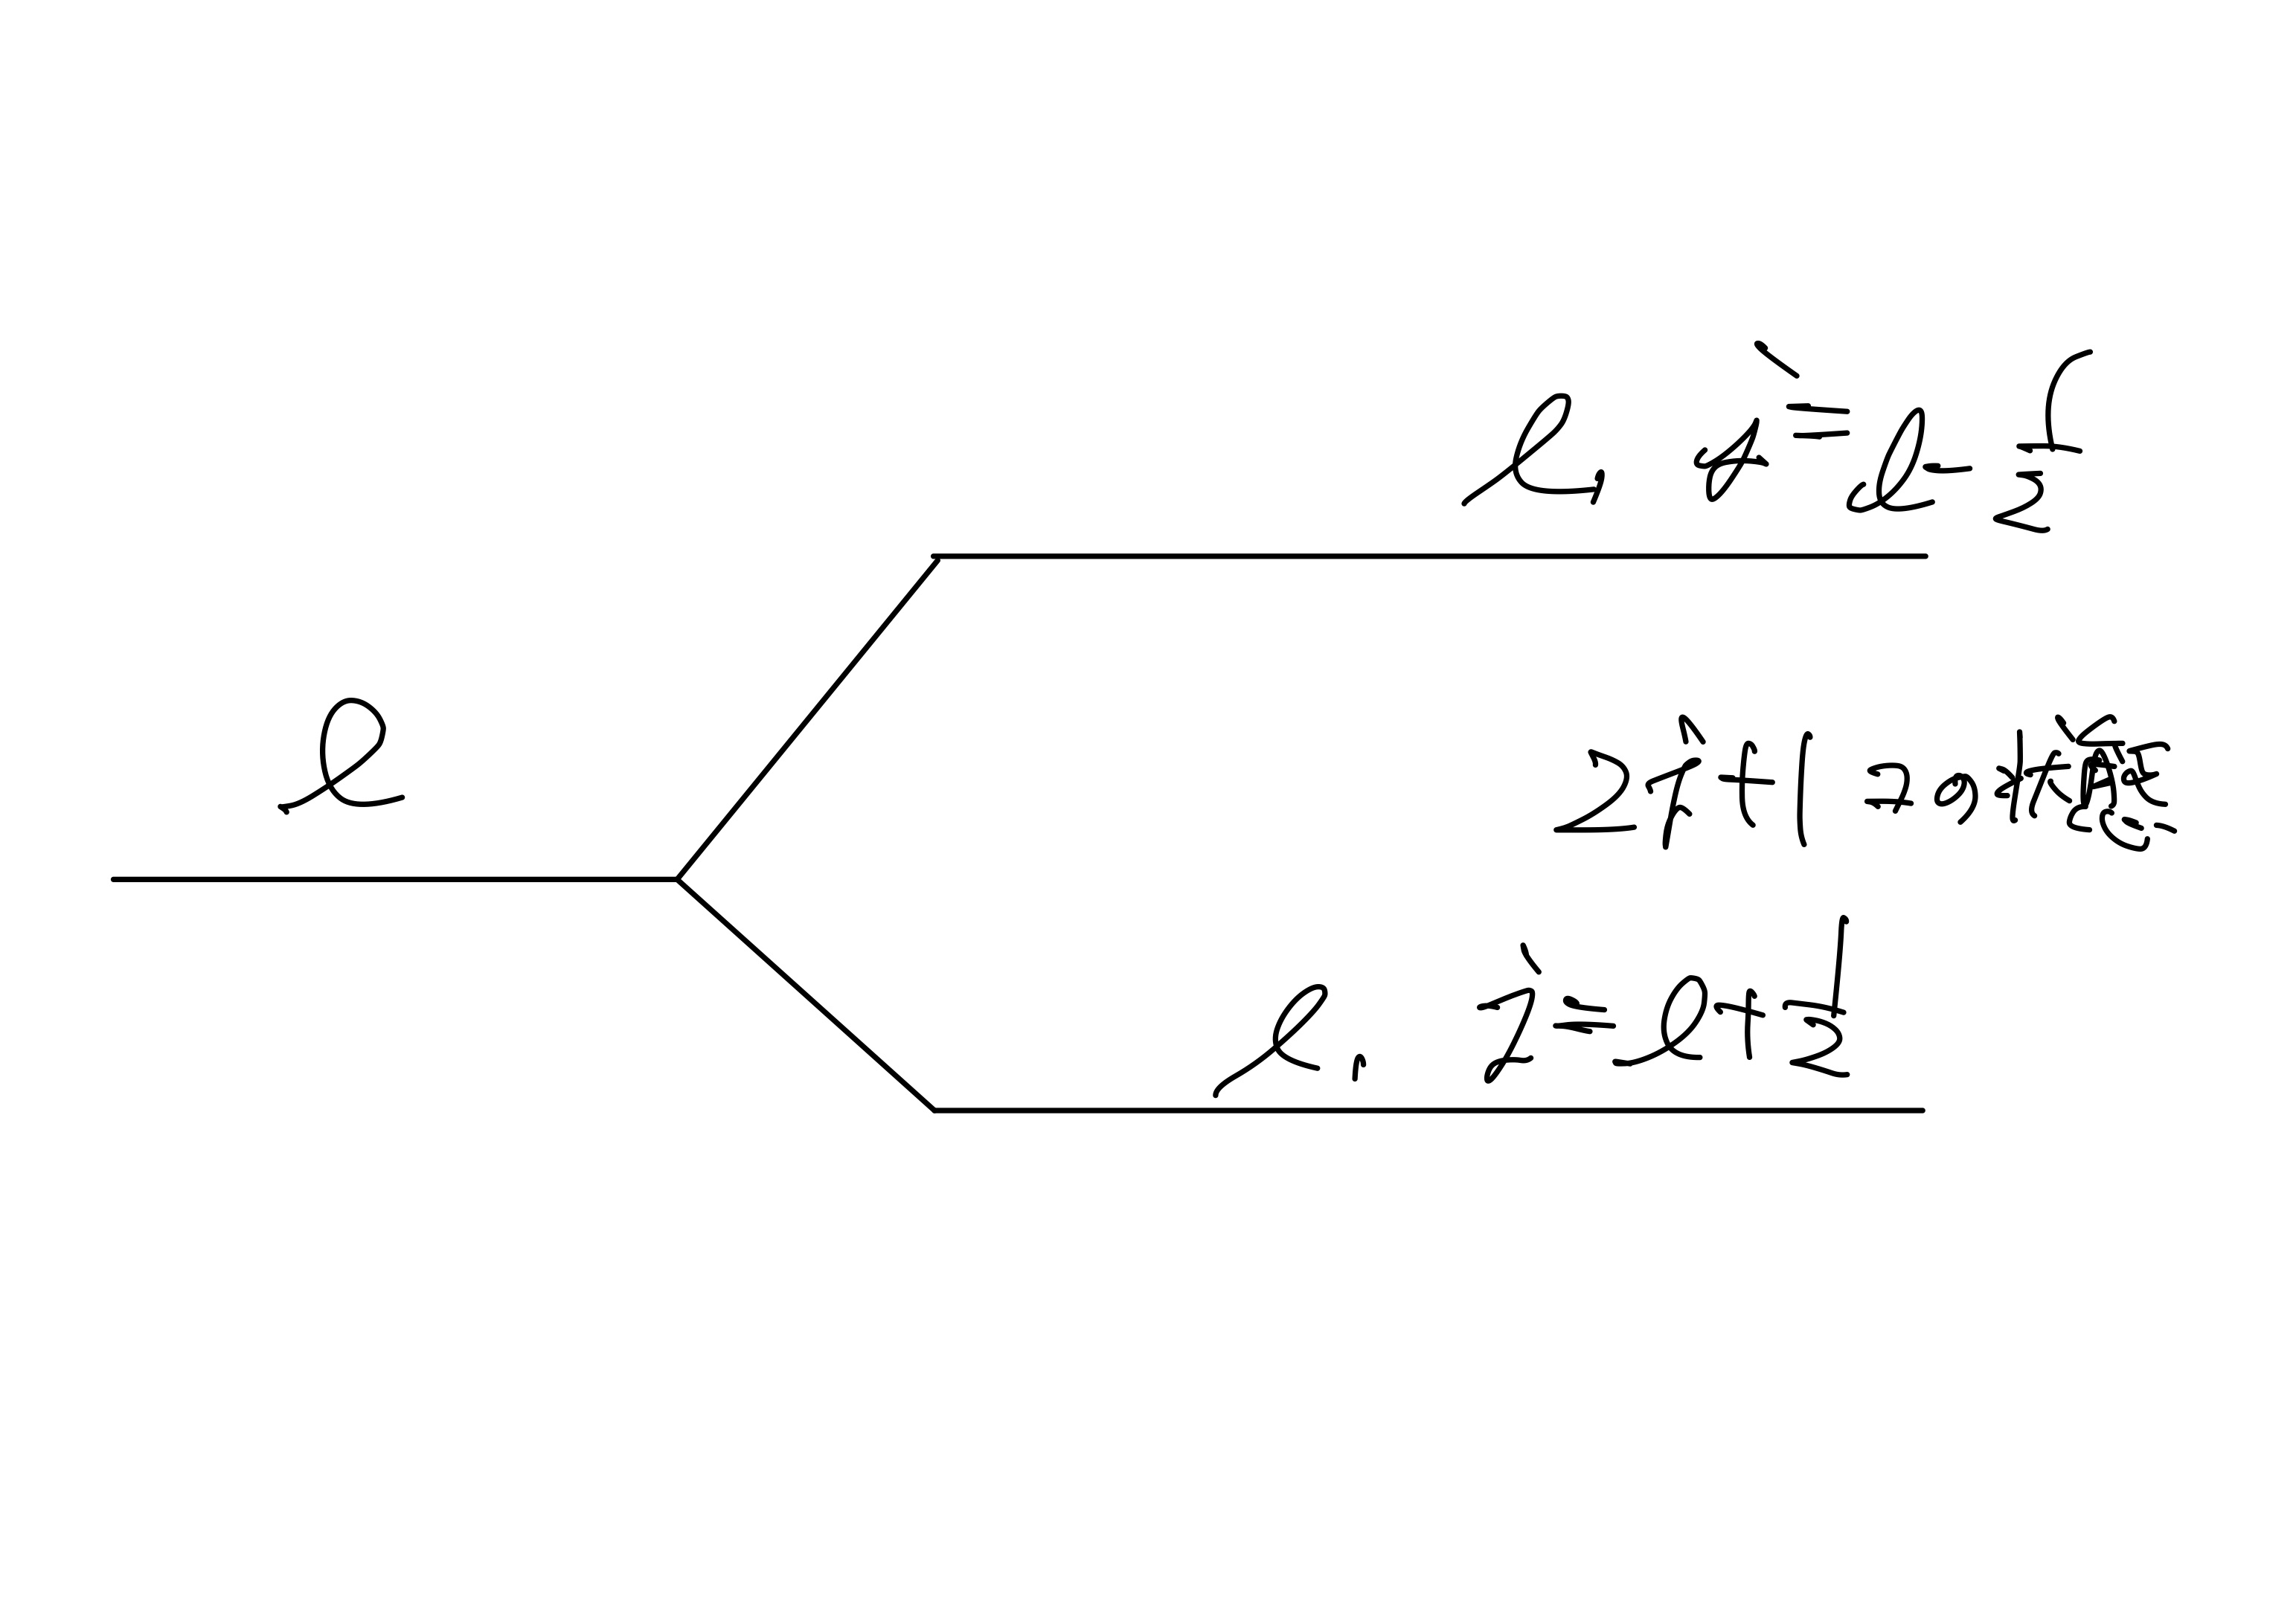
\includegraphics[width=0.5\textwidth]{Fig-4.jpg}
	\caption{スピン軌道相互作用による分裂}
	\label{fig:fig4-Fig-4-jpg}
\end{figure}
以上のことを考慮して$\mathrm{^{24}Mg}$ と$\mathrm{^{27}Al}$ の最低エネルギー状態の全角運動量(核スピン)$j$をもとめる。
それぞれの準位を表にすると表\ref{tab:1}
\begin{table}[H]
	\centering
	\caption{エネルギー準位}
	\label{tab:1}
	\begin{tabular}{ccccc}\hline
	 $N$& $(n_x,n_y,n_z)$ &$nl$  &$D_N$  & $\sum_{N'=0}^{N} D_{N'}$ \\ \hline

	 2& $(n_x,n_y,n_z)$ &$1s,0d$  &12  & 20 \\
	 1& $(100)(010)(001)$ &0p  &6  & 8 \\
	 0& $(000)$ &0s  &2  & 2 \\ \hline
	\end{tabular}
\end{table}
ここで$D_N$  はエネルギー準位縮退度を表している(スピンの自由度2をかけていることに注意)また$N=2n+l$ であり$(n_x,n_y,n_z)$ はデカルト座標出解いたときの量子数である。

いま陽子の数と中性子の数が20におさまるので$N=2$ まで考えれば良い。
例えば$\mathrm{^{24}Mg}$の場合は陽子、中性子ともに12個あり、そのうち$N=0,1$ までで8個埋まり、残りの4個は
$N=2$ のなかで一番小さい準位である$0d$ 軌道のうちスピン軌道相互作用によって分裂した低い方の準位$j=l+\frac{1}{2}=\frac{5}{2}$ に入る。
この低い方の準位は$2j+1=6$ 個あるので残りの4個はこれに収まる。
これが中性子と陽子の場合であるがどちらも4個であり,合計8個である。
ヒントにあるように原子核では核子はペアを組んでお互いの角運動量をなるべく打ち消すように入るのでこの8個が偶数であるために全角運動量の大きさとしてはゼロとなる。
一方で$\mathrm{^{27}Al}$ の場合は同じ$0d$ 軌道のうちスピン軌道相互作用によって分裂した低い方の準位に中性子の方は5個入って陽子の方は6個入ることになるがこのときは陽子が一個多くて一つ余ってしまうので核スピン$\frac{5}{2}$ が残る。

以上まとめると
$^{24}Mg$ の核スピンは0,
$\mathrm{^{27}Al}$ の核スピンは$\frac{5}{2}$ である。

\section{質量をもつベクトル場と核力}
\subsection{}
Euler-Lagrange方程式は
\begin{equation}
\label{eq:21}
\partial_\nu \frac{\partial \mathcal{L}}{\partial (\partial_\nu V_\mu)} -\frac{\partial \mathcal{L}}{\partial V_\mu} =0
.\end{equation}
\[
.\] 
ここでLagragian密度$\mathcal{L}$ は
\[
\mathcal{L}=-\frac{1}{4}(\partial^{\mu}V^{\mu}-\partial^{\nu}V^{\mu})(\partial_\mu V_\nu-\partial_\nu V_\mu)+\frac{1}{2}m^2V_\mu V^{\mu}-gj^{\mu}V_\mu
.\] 
であるがこの内\eqref{eq:21}の第一項の微分に効いてくるのは
\[
-\frac{1}{4}(\partial^{\mu}V^{\mu}-\partial^{\nu}V^{\mu})(\partial_\mu V_\nu-\partial_\nu V_\mu)=-\frac{1}{2}\left[ (\partial_\sigma V_\lambda)(\partial^{\sigma}V^{\lambda})-(\partial_\sigma V_\lambda)(\partial^{\lambda}V^{\sigma}) \right] 
.\] 
まずこの部分の計算について実行する。
ここで上付きの添字を下ろす操作を二回行うと符号は変わらないことに注意して
\begin{align*}
	-\frac{1}{2}\partial_\nu \frac{\partial }{\partial (\partial_\nu V_\mu)} \sum_{\sigma,\lambda}^{} \left[ (\partial_\sigma V_\lambda)(\partial_{\sigma}V_{\lambda})-(\partial_\sigma V_\lambda)(\partial_{\lambda}V_{\sigma}) \right] &=-\frac{1}{2}\partial_\nu \frac{\partial }{\partial (\partial_\nu V_\mu)} \left[ (\partial_\nu V_\mu)^2-2(\partial_\nu V_\mu)(\partial_\mu V_\nu) \right]   \\
	&= -\partial_\nu \partial^{\nu}V^{\mu}+\partial_\nu \partial_\mu V_\nu \\
	&= -\Box V^{\mu}+\partial^{\mu} \partial_\nu V^{\nu}\\
.\end{align*}
なお最後の式は偏微分をいれかえた。
一方で\eqref{eq:21}の第二項に効いてくるのは$\mathcal{L}$ のうち
\[
\frac{1}{2}m^2V_\mu V^{\mu}-gj^{\mu}V_\mu
.\] 
の部分であり、計算すると
\[
\frac{\partial }{\partial V_\mu} \left( \frac{1}{2}m^2V_\nu V^{\nu}-gj^{\nu}V_\nu \right) =m^2V^{\mu}-gj^{\mu}
.\] 
以上まとめると場の方程式は
\begin{equation}
\label{eq:22}
\Box V^{\mu}-\partial^{\mu}\partial_\nu V^{\nu}+m^2V^{\mu}-gj^{\mu}=0
.\end{equation}
ここで\eqref{eq:22}に$\partial_\mu$ を作用させることにより第1項と第2項がキャンセルして
\[
m^2\partial_\mu V^{\mu}=g\partial_\mu j^{\mu}=0
.\] 
ここで$j^{\mu}$ が保存する4元カレントであることを使った。
したがって
\[
\partial_\mu V^{\mu}=0
.\] 
である。このとき\eqref{eq:22}は次のように書き直せる。
\begin{equation}
\label{eq:23}
(\Box+m^2) V^{\mu}=gj^{\mu}
.\end{equation}

\subsection{}
\eqref{eq:23}を解く。
今$g$ の電荷をもった2つのsourceが距離$r$ だけ離れておいてあるので
一つの電荷に着目してそれが作るポテンシャル$V(r)$ に電荷$g$ 
をかけたもの$U(r)$というポテンシャルを考えればよい。
\eqref{eq:23}は
\begin{equation}
\label{eq:24}
(\nabla ^2-m^2)V=g\delta (\bm{r})
.\end{equation}
となりこれを解くと
\[
V=\frac{g e^{-mr}}{4\pi r}
.\] 
したがって
\[
U(r)=\frac{g^2e^{-mr}}{4\pi r}
.\] 
\subsection{}
ポテンシャルが斥力になるのは
\eqref{eq:24}の右辺がマイナスになっていることからわかる。(電磁気とおなじ)。
また今質量\SI{782}{MeV}の中性のベクトル中間子$\omega$ を
考えると
斥力の典型的な到達距離は
\[
\frac{1}{m}=\frac{1}{\SI{782}{MeV}}\to \frac{\hbar c}{m}=\frac{197}{782}\simeq \SI{0.3}{fm}
.\] 
ここで$\hbar c=\SI{197}{MeV .fm}$ であることを
用いた。
\section{クォーク$\cdot $グルーオン$\cdot $ プラズマとビッグバン元素合成}
\subsection{}\label{3-1}
まず相対論的なボソン気体について述べる。
大分配関数が
\[
\Xi=\prod_k \sum_{N(k)=0}^{\infty} \exp (-\beta E(k)N(k)) ,\quad(\beta=\frac{1}{T})
.\] 
ここで今は相対論的粒子を考えているので
\[
E^2=k^2+m^2\simeq k^2 \quad \therefore E(k)=k
.\] 
このとき
\[
\Xi=\prod _k \frac{1}{1-e^{-k /T}}
.\] 
また分布関数は
\[
f(k)=\frac{1}{e^{k /T}-1}
.\] 
であり、エネルギー密度$\varepsilon$を求めると
\[
\varepsilon=g \int_{0}^{\infty} \left( \frac{1}{2\pi} \right) ^3 kf(k)dk^3=  2 \int_{0}^{\infty} \left( \frac{1}{2\pi} \right) ^3 \frac{k}{e^{k /T}-1}4\pi k^2dk
.\] 
ここで$g$ はスピン自由度で$g=2$ とした。
整理して
\[
\varepsilon=\frac{T^{4}}{\pi^2}\int_{0}^{\infty} \frac{x^3}{e^{x}-1} =\frac{\pi^2}{15}T^{4}
.\] 
1自由度あたりだと
\[
\varepsilon=\frac{\pi^2}{30}T^{4}
.\] 
また統計力学の式より
\[
	-pV=J=-T\log \Xi
.\] 
であるので
\begin{align*}
	pV&= T\log \Xi \\
	&= -gTV \int_{0}^{\infty}\left( \frac{1}{2\pi} \right) ^3\log (1-e^{-k /T})d^3k   \\
	&=- \frac{1}{\pi^2}TV \int_{0}^{\infty} k^2\log (1-e^{-k /T})dk  \\
	&= -\frac{T^{4}}{\pi^2}V \int_{0}^{\infty} x^2\log (1-e^{-x})dx  \\
	&= -\frac{T^{4}}{\pi^2}V\left[ \frac{x^3}{3}\log (1-e^{-x}) \right] _{0}^{\infty}+\frac{T^{4}}{3\pi^2}V \int_{0}^{\infty} \frac{x^3}{(e^{x}-1)}dx  \\
	&=\frac{\pi^2}{45}T^{4}V  \\
.\end{align*}
すなわち1自由度辺りだと
\begin{equation}
\label{eq:p3}
p=\frac{\pi^2}{90}T^{4}
.\end{equation}
以上より
\begin{equation}
\label{eq:31}
	\varepsilon=3p=\frac{\pi^2}{30}T^{4}
.\end{equation}

続いて相対論的なフェルミ粒子について同じように計算する。
まず大分配関数は
\[
\Xi=\prod _k (1+e^{-k /T})
.\] 
分布関数は
\[
f(k)=\frac{1}{e^{k /T}+1}
.\] 
したがってエネルギー密度は
%%%%%%%%%%%%%%%%%%%%%%%%%5jk
\[
\varepsilon=g \int_{0}^{\infty} \left( \frac{1}{2\pi} \right) ^3 kf(k)dk^3=  2 \int_{0}^{\infty} \left( \frac{1}{2\pi} \right) ^3 \frac{k}{e^{k /T}+1}4\pi k^2dk
.\] 
ここでも$g$ はスピン自由度で$g=2$ とした。
整理して
\[
\varepsilon=\frac{T^{4}}{\pi^2}\int_{0}^{\infty} \frac{x^3}{e^{x}+1} =\frac{7}{120}\pi^2T^{4}
.\] 
1自由度あたりだと
\[
\varepsilon=\frac{7}{240}\pi^2T^{4}
.\] 
再び統計力学の式
\[
	-pV=J=-T\log \Xi
.\] 
を使って

\begin{align*}
	pV&= T\log \Xi \\
	&= gTV \int_{0}^{\infty}\left( \frac{1}{2\pi} \right) ^3\log (1+e^{-k /T})d^3k   \\
	&= \frac{1}{\pi^2}TV \int_{0}^{\infty} k^2\log (1+e^{-k /T})dk  \\
	&= \frac{T^{4}}{\pi^2}V \int_{0}^{\infty} x^2\log (1+e^{-x})dx  \\
	&= \frac{T^{4}}{\pi^2}V\left[ \frac{x^3}{3}\log (1+e^{-x}) \right] _{0}^{\infty}+\frac{T^{4}}{3\pi^2}V \int_{0}^{\infty} \frac{x^3}{(e^{x}+1)}dx  \\
	&=\frac{7}{360}\pi^2T^{4}V  \\
.\end{align*}
すなわち1自由度辺りだと
\[
p=\frac{7}{720}\pi^2T^{4}
.\] 
以上より
\begin{equation}
\label{eq:32}
	\varepsilon=3p= \frac{7}{240}\pi^2T^{4}=\frac{7}{8}\times \frac{\pi^2}{30}T^{4}
.\end{equation}
となりボソン気体のときと比べて$7 /8$ だけ変わる。
\subsection{}
\eqref{eq:p3}の結果と\eqref{eq:32}のようにフェルミ気体では結果が$7 /8$ 倍されること、およびスピン、フレーバー、カラーの自由度を考えることにより
\[
	P_\text{QGP} =d_\text{QGP} \frac{\pi^2}{90}T^{4}
.\] 
\begin{align*}
	d_\text{QGP} &=2_\text{spin} \times (N_c^2-1)+\frac{7}{8}\times 2_\text{spin} \times 2_{q\overline{q}}\times N_c\times N_f \\
	&= 2\times 8+\frac{7}{8}\times 2\times 2\times 3\times 3=\frac{95}{2} \\
.\end{align*}
ここで$N_c=3$ はカラーの自由度であり、$N_f$ はフレーバーの自由度、$2_{q\overline{q}}$ は粒子反粒子の自由度で、$2_\text{spin} $ はスピンの自由度である。
したがって
\[
P_\text{QCD} =\frac{95}{2}\frac{\pi^2}{90}T^{4}=\frac{19}{36}\pi^2T^{4}
.\] 
\subsection{}
まず陽子の質量が我々の住んでいる宇宙と同じである場合にどのように$\mathrm{He}$ と$\mathrm{H}$ の存在比が$\mathrm{H}:\mathrm{He}=3:1$になるかについて確認する。
平衡状態において陽子と中性子の存在比は
	
\begin{equation}
\label{eq:hei}
	\left( \frac{n_n}{n_p} \right)_\text{eq}  =e^{ \frac{-\Delta m}{T}} \quad(\Delta m=m_n-m_p=\SI{1.3}{MeV})
.\end{equation}
と書ける。温度が下がると中性子の割合が減っていくがいつまでも減り続けるかというとそうではなく、宇宙
膨張の効果を加味してハップル膨張率とニュートリノ反応率との競合で決まる温度あたりでニュートリノ脱結合がおきてそのあたりで反応率はゆっくりになる。このあたりの温度はfreez out temperature とよばれ$T=\SI{0.7}{MeV}$ あたりである\cite{5}。これを\eqref{eq:hei}にいれて
	\begin{equation}
	\label{eq:16}
	\left( \frac{n_n}{n_p} \right)_\text{eq}  =e^{ \frac{-\Delta m}{T}} \simeq \frac{1}{6}
	.\end{equation}
ここからさらに元素合成($t\sim \SI{3}{min}$)が起こり
この3分間でさらに
\[
	n\to p+e^{-}+\nu_e
\] 
なる反応によって$n$ が減る。
この崩壊時間$\tau$ は$\tau=\SI{880}{s}$\cite{5} ほどであり、これが
3分の間に起こるので
\begin{equation}
\label{eq:time}
\frac{n}{p}\simeq \frac{1}{6}\exp (-\frac{t}{\tau})=\frac{1}{6}\exp \left( -\frac{\SI{180}{s}}{\SI{880}{s}} \right) \simeq \frac{1}{7}
.\end{equation}
ここから$\mathrm{He}$ と$\mathrm{H}$ の存在比が$\mathrm{H}:\mathrm{He}=3:1$になることが導かれる。

ここまでの議論を仮に陽子の質量が$\SI{1.0}{MeV}$ 大きかった大きかったとすると
\[
\Delta m= m_n-m_p=\SI{0.3}{MeV}
.\] 
となり、
\eqref{eq:16}は
\begin{equation}
\label{eq:16kai}
	\left( \frac{n_n}{n_p} \right)_\text{eq}  =e^{ \frac{-\Delta m}{T}} \simeq e^{ -\frac{\SI{0.3}{MeV}}{\SI{0.7}{MeV}}} \simeq \frac{1}{1.5}
.\end{equation}
さらに\eqref{eq:time}より
\begin{equation}
\label{eq:timekai}
\frac{n}{p}\simeq \frac{1}{6}\exp (-\frac{t}{\tau})=\frac{1}{1.5}\exp \left( -\frac{\SI{180}{s}}{\SI{880}{s}} \right) \simeq \frac{1}{1.9}
.\end{equation}
したがって$n:p=1:2$ である。
つまりこのときの$\mathrm{He},\mathrm{H}$ 比は
\[
\mathrm{He}:\mathrm{H}=2:1
.\] 
別の言い方をすると$\mathrm{He}:66.6\%$で$\mathrm{H}:33.3\%$ である。
\section{超新星におけるニュートリノ}
\subsection{}\label{4-1}
ニュートリノと原子核の反応の確率振幅は弱い相互作用の大きさ結合定数$G_F$ に比例する。したがって断面積$\sigma$ は$G_F$ に2乗に比例する。また散乱振幅は$A$ に比例するので$\sigma$ は$A^2$ に比例する。
後は次元解析によってニュートリノのエネルギー$E_\nu$ を含めると
数係数は無視して
\[
\sigma=A^2G_F^2E_\nu^2
.\] 
\subsection{}\label{4-2}
超新星コアでは物質密度は十分に高いため、電子は相対論的であり縮退したフェルミ準位ガスの状態にある。
このとき電子の化学ポテンシャル$\mu_e$ を求める。
まず
\[
N_e=g \int_{0}^{p_F} \frac{V}{(2\pi)^3} d\bm{p}=g \int_{0}^{p_F} \frac{V}{(2\pi)^3}4\pi p^2 dp=g \frac{V p_F^3}{6\pi^2} 
.\] 
ここで$g$ はスピンの自由度で今の場合は$g=2$ である。$p_F$ はフェルミ運動量であるが、相対論的で今、自然単位系を用いているので
\[
\mu_e=p_F
.\] 
である。したがって$N_e /V=n_e$ として
\begin{equation}
\label{eq:41}
\mu_e=(3\pi^2n_e)^{1 /3}
.\end{equation}
ここで電気的中性条件により核子密度を$n_B$として
\begin{equation}
\label{eq:42}
n_e=Y_e n_B=Y_e \frac{\rho}{m_N}
.\end{equation}
したがって\eqref{eq:42}を\eqref{eq:41}に代入して
\begin{equation}
\label{eq:43}
\mu_e=\left( 3\pi^2 \frac{\rho}{m_N}Y_e \right) ^{1 /3}
.\end{equation}
\subsection{}\label{4-3}
まず原子核数密度$n_A$ は
\[
n_A=\frac{n_B}{A}=\frac{\rho}{m_N A}
.\] 
ニュートリノの平均自由行程$l_\text{mfp} $ は
\begin{equation}
\label{eq:44}
	l_\text{mfp} =\frac{1}{\sigma n_A}=\frac{1}{(A^2G^2_FE^2_\nu)(\rho /m_N A)}
.\end{equation}
ここでニュートリノのエネルギー$E_\nu$ は電子の化学ポテンシャル$\mu_e$にほぼ等しいので$E_\nu=\mu_e$として\eqref{eq:43}を\eqref{eq:44}に代入すると
\begin{equation}
\label{eq:45}
	l_\text{mfp} = \frac{1}{AG_F^2(3\pi^2 Y_e)^{2 /3}}\left( \frac{m_N}{\rho} \right) ^{5 /3}
.\end{equation}
$\rho \sim  \SI{e 14}{g.cm^{-3}}$ の超新星コアの領域で
$A$ と$Y_e$ については原子核のうちで最も安定な$\mathrm{^{56}Fe}$ での値を用いると$A=56$、$Y_e=0.46$。フェルミ定数$G_F \sim \SI{e-5}{GeV^{-2}}=\SI{e-11}{MeV}$ と
核子質量$m_N=\SI{939}{MeV}$ の値を用いて\eqref{eq:45}をオーダー評価する。
まず $\rho$ の部分について
\begin{equation}
\label{eq:46}
	\rho\sim \SI{e14}{g.cm^{-3}}=\SI{e-28}{kg.fm^{-3}}=\frac{\SI{e-28}{kg}}{(\SI{1}{fm})^{3}}\sim \frac{\SI{56}{MeV}}{(\SI{5.1e-3}{MeV^{-1}})^{3}}\sim \SI{4.2 e8}{MeV^{4}}
.\end{equation}
\newpage
ただしここで
\[
\SI{1}{kg}\to  \SI{1}{kg}  \times \left. (\SI{3e 8}{m.s^{-1}}) \right|_\mathrm{J}  \times \left. \frac{1}{1.602\times 10^{-19}} \right| _\mathrm{eV}\times \left. 10^{-6} \right| _\mathrm{MeV}
.\] 
\[
\SI{1}{fm}\to \SI{1}{fm}\times \left. \frac{1}{197} \right| _\mathrm{MeV}
.\] 
であることを用いた。
この\eqref{eq:46}を考慮して\eqref{eq:45}は
\[
	l_\text{mfp} \sim \frac{1}{56\times (3\pi^2\times 0.49)^{2  /3}}\times \frac{1}{(\SI{e-11}{MeV^{-2}})^{2}}\times \left( \frac{\SI{939}{MeV}}{\SI{4.2e 8}{MeV^{4}}} \right) ^{5 /3}\sim \SI{1.15e 10}{MeV^{-1}} 
.\] 
これを\si{mm}の単位で書くと
\[
l_\text{mfp} \sim 1.15\times 10^{10}\times 197=\SI{2.3e 12}{fm}=\SI{2.3}{mm}
.\] 
\subsection{}
余力がないのでやりませんでした。
\begin{thebibliography}{99}
	\bibitem{1} 慶應原子核物理授業ノート
	\bibitem{2}核分裂の物理学\url{https://www.jstage.jst.go.jp/article/jaesjb/58/11/58_664/_pdf/-char/ja}、2022年07月20日閲覧
	\bibitem{3} 川村嘉春、「基礎物理から理解するゲージ理論」、サイエンス社、2017年
	\bibitem{4} Mathematica
	\bibitem{5}physics stack exchange,"What is the reason for the shift in balance between neutrons and protons in the early universe?" 
	\url{https://physics.stackexchange.com/questions/399297/what-is-the-reason-for-the-shift-in-balance-between-neutrons-and-protons-in-the}、2022年07月21日閲覧
	\bibitem{6}ウィキペディア、「クォークグルーオンプラズマ」、\url{https://ja.wikipedia.org/wiki/%E3%82%AF%E3%82%A9%E3%83%BC%E3%82%AF%E3%82%B0%E3%83%AB%E3%83%BC%E3%82%AA%E3%83%B3%E3%83%97%E3%83%A9%E3%82%BA%E3%83%9E}、2022年07月24日閲覧
	\bibitem{7}松本憲樹、「ニュートリノ振動と質量問題」、\url{https://core.ac.uk/download/pdf/70292931.pdf}、2022年07月24日閲覧
	\bibitem{8}住吉光介、「原子核から読み解く超新星爆発の世界」、共立出版、2018年

\end{thebibliography}
\end{document}
